\documentclass{article}
\usepackage[utf8]{inputenc}
\usepackage{caption}
\usepackage{graphicx}
\usepackage{listings}
\usepackage{cite}
\usepackage{amsmath}

\usepackage[framed,numbered,autolinebreaks,useliterate]{mcode}

\bibliographystyle{a}

\title{ENGN4528 Computer Vision Clab4 Report}
\author{Zhipeng Bao ~~ u6600985}
\date{May 2018}



\begin{document}

\maketitle
\section*{Introduction}
For this task, I want to try both of the tasks. The primary task I chose is the Task 1: CNN for MNIST handwriting digit recognition. And the secondary task is the camera resectioning.

\section*{Primary Task:  CNN for MNIST handwriting digit recognition}

\subsubsection*{Basic experimental environment}

For this task, I use a python package named \emph{keras} to help build the model. It is released by Google and also based on tensorflow. Besides, I use a GPU server to help training. The platform I used was Ubuntu 16.04.4 with 2 GeForce TITAN X. To train more powerful models. As required, I select 10,000 samples as training set and 10,000 samples as test set. I think the samples are set randomly in the file so I just chose the first 10,000 samples as training data.

I also divided the training data into two parts, 80\% of them are used as the training set and 20\% of them are used as the validation set. To get the most accurate result, I apply an early-stopping method ~\cite{early_stopping}. The early-stopping method will stop when the monitored index does not go up/down. 

I built three kinds of models in total. This first is a Fully-connected model, the second is a Conv-Dense model and the last one is a Conv-Conv-Dense model.

There are also some constant variables in my codes. They are:

\begin{enumerate}
    \item \textbf{$epoches = 100$} That is the program will train 100 epoches if not been stopped(early stopping). \item \textbf{$train_patience = 6$} That is if the monitored index, in this case is val loss, does not go better in 6 epoches, stop training.
    \item \textbf{$num_class = 10$} 10 classes of handwritings in total.
    \item \textbf{$img_rows, img_cols = (28,28)$} The shape of the input images.
    
\end{enumerate}


\subsubsection*{Fully-Connected model}
Figure 1 shows the the model architecture. There are three hidden layers in total. 

\begin{figure}[htbp]
    \centering
    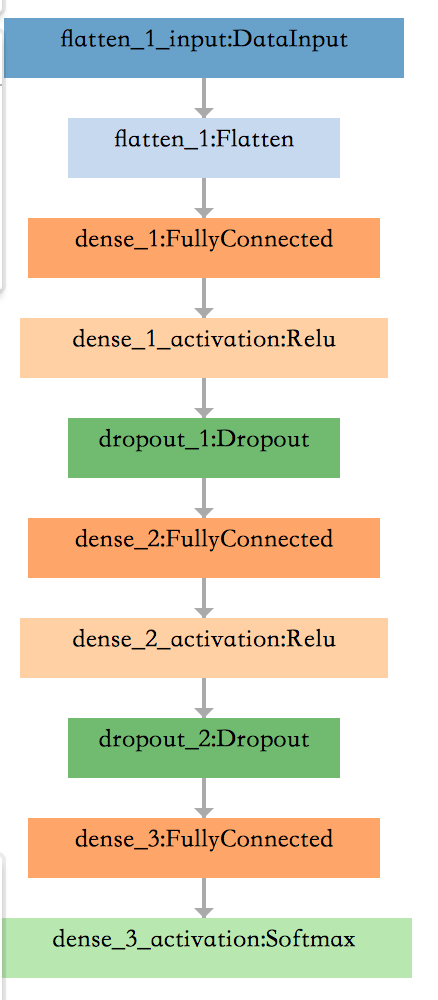
\includegraphics[scale = 0.6]{fig1.png}
    \caption{Model Architecture for Dense Model}
    \label{fig1}
\end{figure}


In this model, I have 5 hyper parameters: $batch_size$, $lr$, $hidden_layer1$, $hidden_layer2$ and $Dropout_rate$. For these parameters, $lr$ means learning rate and $Dropout_rate$ means the dropout rate for dropout layers which is used to avoid overfitting~\cite{dropout} .


I firstly adjust all the parameters until get the best model. Table 1 shows the value of these parameters and final results. When doing this process, I choose another optimizer: Adadelta. It will have less influence for the test of required optimizers.

\begin{table}[ht]
    \caption{Values of parameters}
    \centering
    \begin{tabular}{|l|c|}
    \hline
         Parameters & values \\ \hline
         lr & 0.1 \\
         batch\_size & 150 \\
         hidden\_layer1 & 512  \\
         hidden\_layer2 & 256\\
         Dropout\_rate & 0.3 \\ \hline
    \end{tabular}
    \label{table1}
\end{table}

Then I switch the optimizer to SGD, ADAM and ADAGRAD. Table 2 shows the related results by different optimizers.

\begin{table}[ht]
    \caption{Result on 3 optimizers}
    \centering
    \begin{tabular}{|l|c|c|c|c|}
    \hline
         Optimizer  & Adaelta & SGD & Adam & Adagrad\\ \hline
         Convergence Rate(epoches) &  93 &46 & 23 &  200\\ \hline
         train acc & 98.86\% & 98.64\% & 99.25\% & 98.10\%\\
         train loss & 0.0447 & 0.0503 & 0.0245 & 0.0756\\ \hline
         val acc &  94.90\% & 94.90\% & 95.60\% & 94.00\% \\
         val loss & 0.1800 &0.1802 & 0.1703 & 0.1997 \\ \hline
         test acc & 95.66\% & 95.29\% & 96.03\% & 94.94\% \\
         test loss & 0.1532 & 0.1604 & 0.1507 &  0.1680\\ \hline
    \end{tabular}
    \label{table2}
\end{table}

What needs to be confirm is that For Adam optimizer, the learning rate is 0.001 and for Adagrad optimizer, the learning rate is 0.01 as they will not work with lr as 0.1. Figure 2 to Figure 6 shows the loss and acc curve for the four optimizers.


\begin{figure}[htbp]
\centering
\begin{minipage}[t]{0.48\textwidth}
\centering
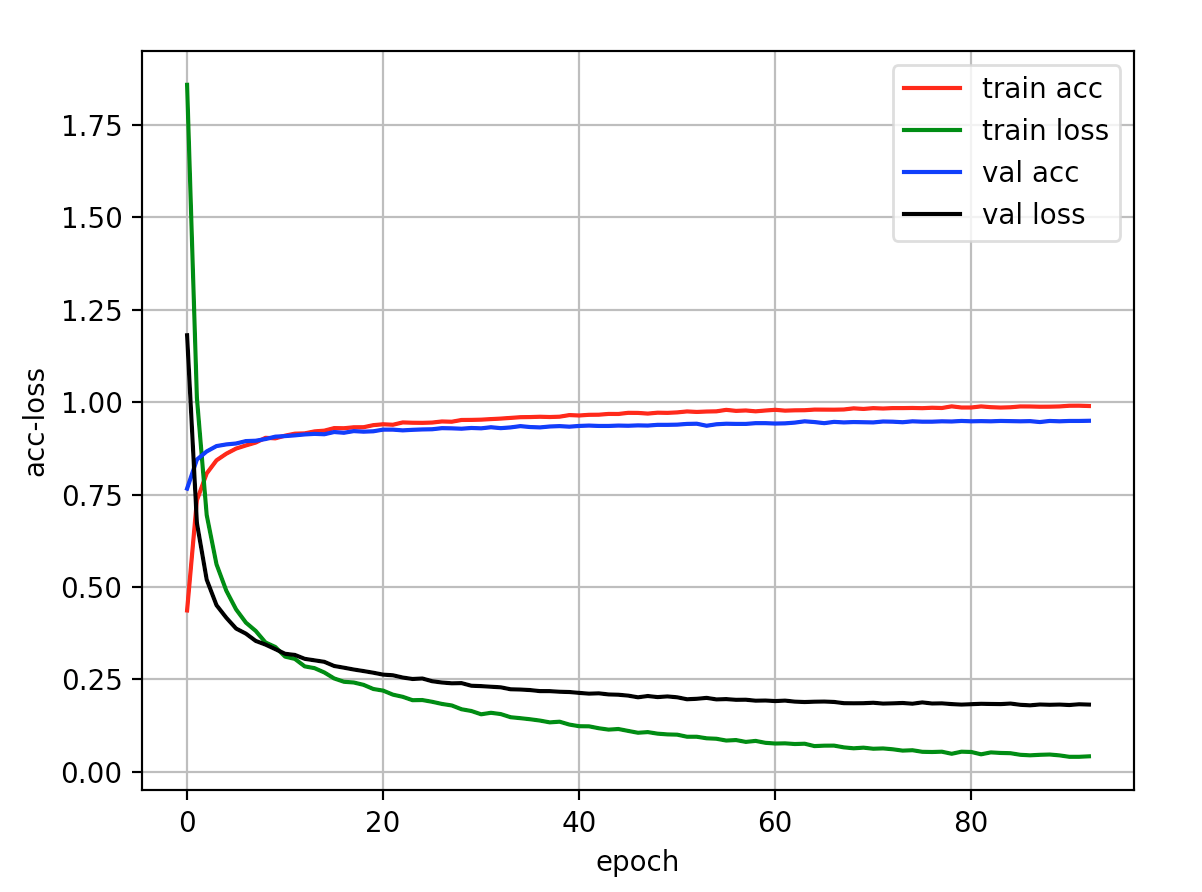
\includegraphics[scale = 0.3]{adaelta.png}
\caption{Loss and Accuracy curve for Adadelta optimizer}
\end{minipage}
\begin{minipage}[t]{0.48\textwidth}
\centering
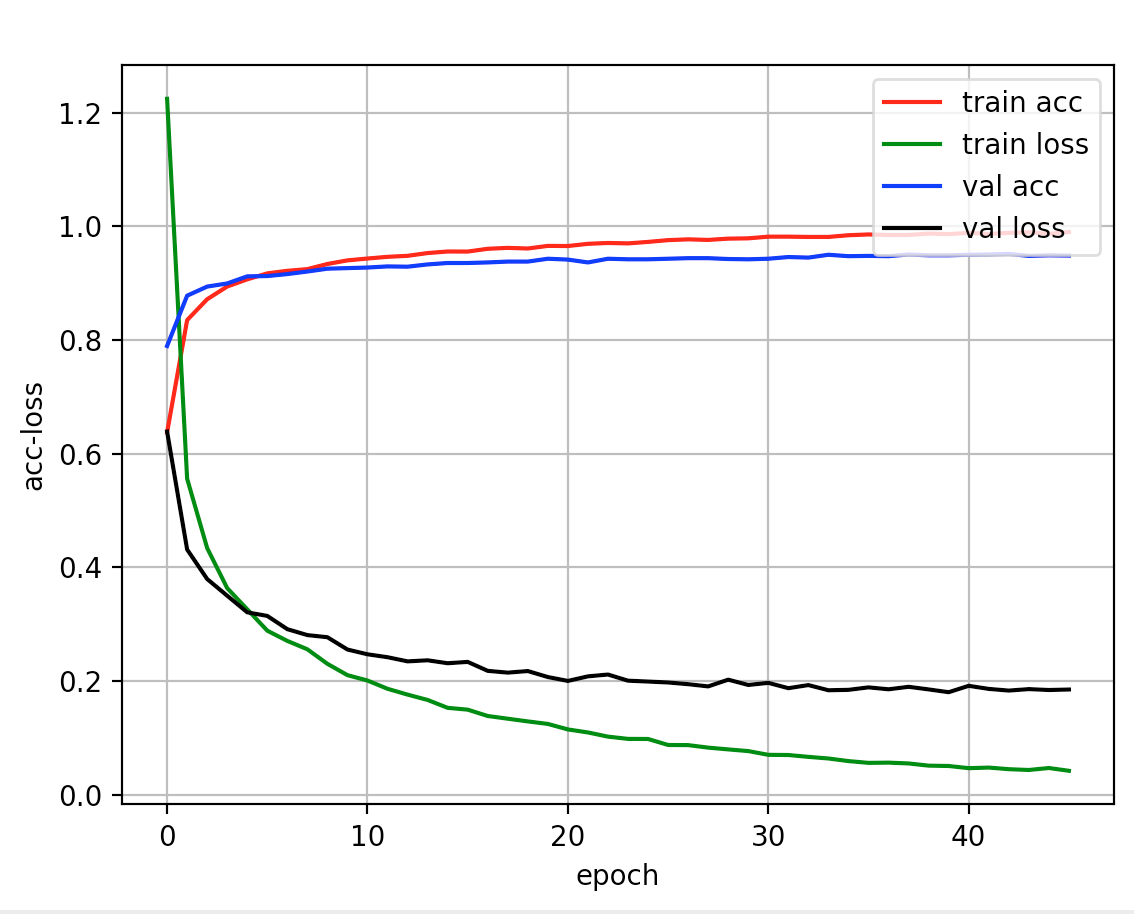
\includegraphics[scale = 0.3]{sgd.png}
\caption{Loss and Accuracy curve for SGD optimizer}
\end{minipage}
\end{figure}

\begin{figure}[htbp]
\centering
\begin{minipage}[t]{0.48\textwidth}
\centering
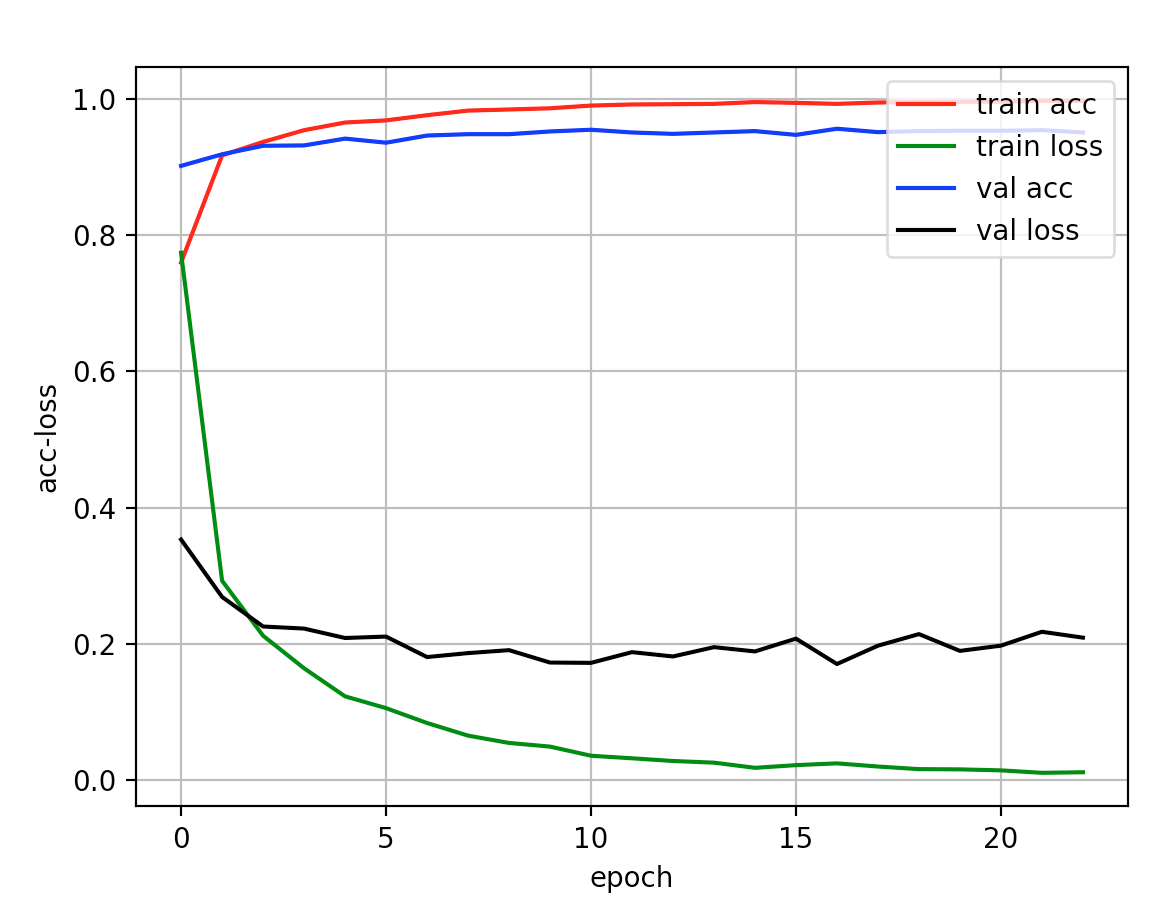
\includegraphics[scale = 0.3]{adam_0_001.png}
\caption{Loss and Accuracy curve for Adam optimizer (lr = 0.001)}
\end{minipage}
\begin{minipage}[t]{0.48\textwidth}
\centering
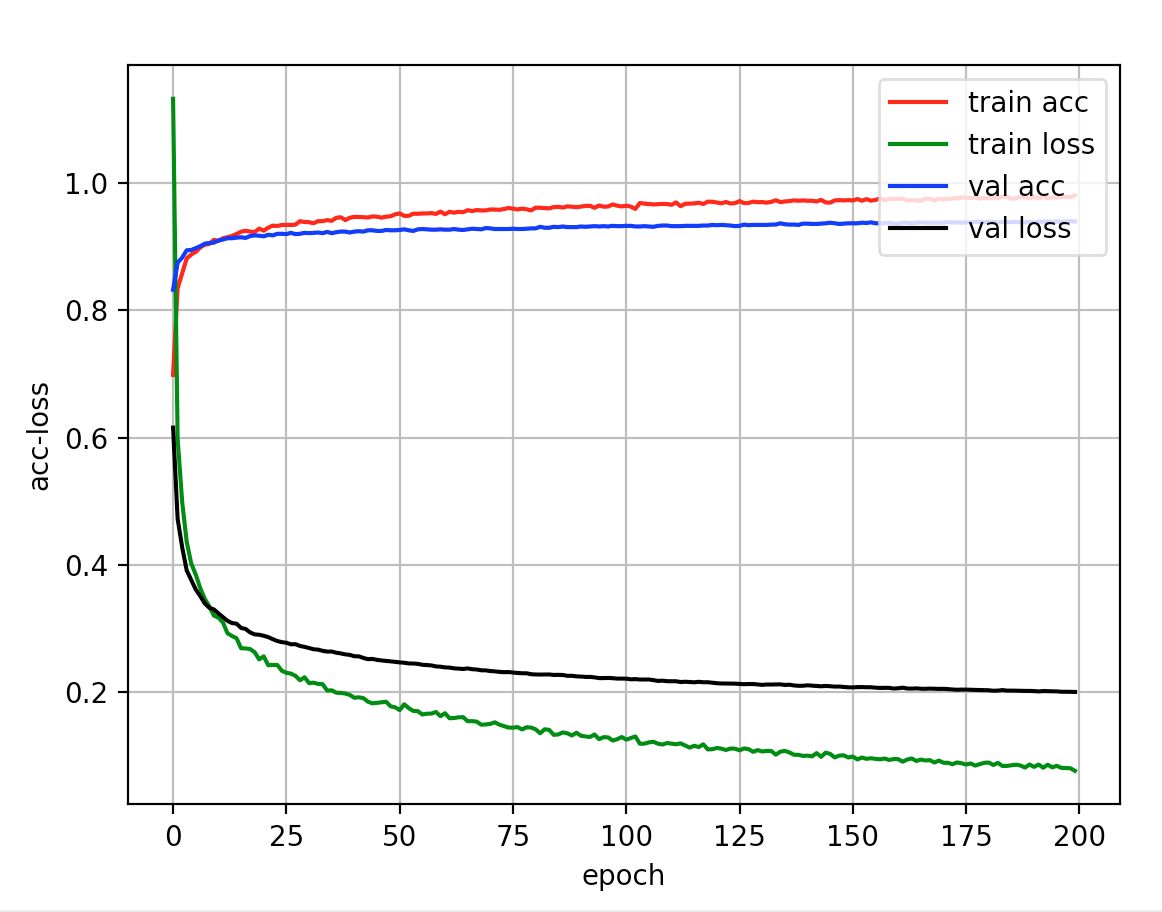
\includegraphics[scale = 0.3]{adagrad_0_01.png}
\caption{Loss and Accuracy curve for Adagrad optimizer (lr = 0.01)}
\end{minipage}
\end{figure}

\begin{figure}[htbp]
    \centering
    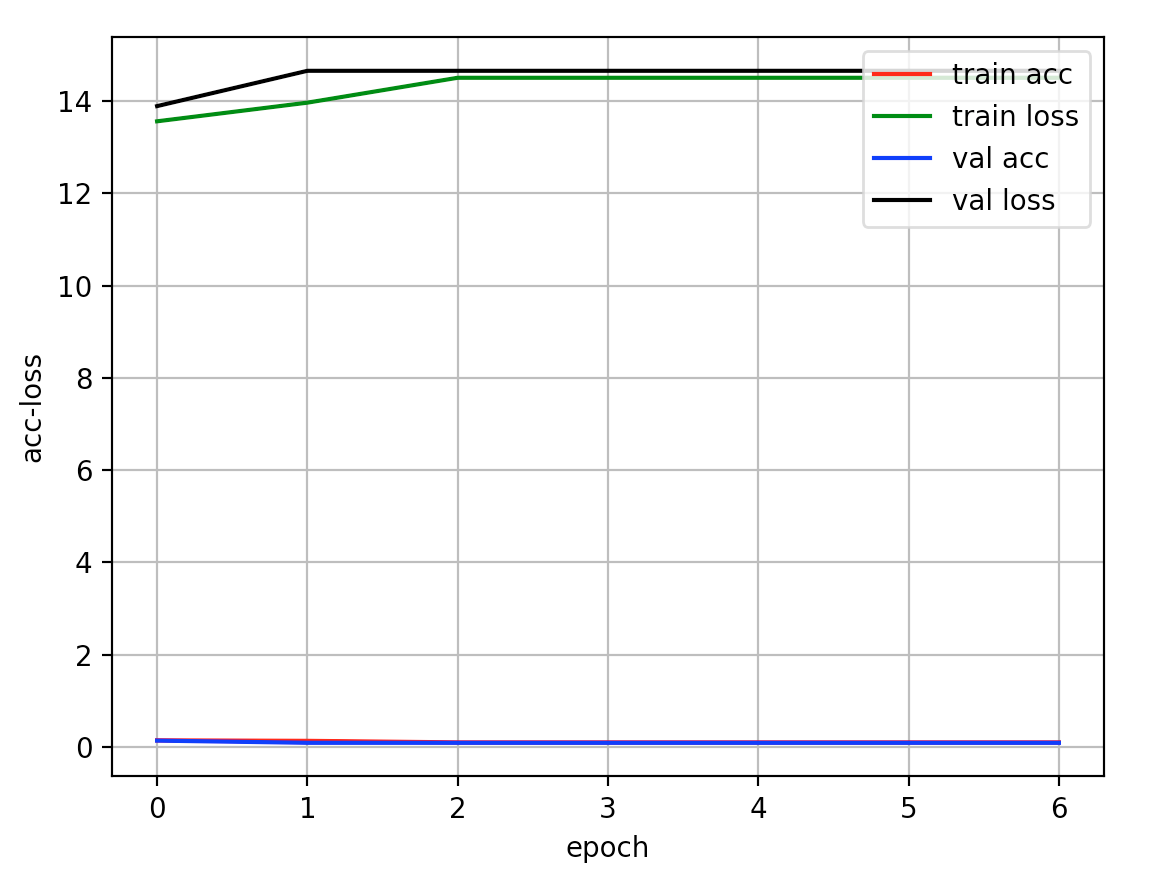
\includegraphics[scale = 0.5]{adam.png}
    \caption{Loss and Accuracy curve for Adagrad optimizer (lr = 0.1)}
    \label{fig6}
\end{figure}

Figure 6 shows the result of Adam optimizer with learning rate as 0.1. The model cannot find the optimal with such a big learning rate. So does Adagrad optimizer. To improve the model, we can use the default keras learning rate which could change among different optimizers.

For this party, We can see from the figures and Table 2 that adam optimizer work best for this model. It can solve the optimization with a smaller learning rate which says it can find the most optimal destination each step. 



\subsubsection*{Conv-Dense Model}

Figure 7 shows the the model architecture of Conv-Dense model. There are three hidden layers in total. 

\begin{figure}[htbp]
    \centering
    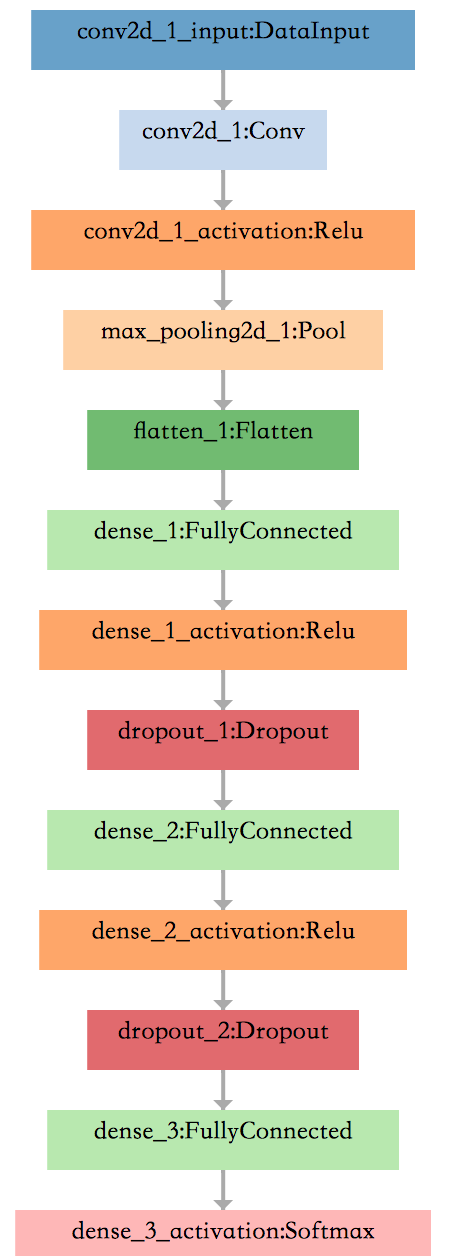
\includegraphics[scale = 0.5]{model2.png}
    \caption{Model architecture for conv-dense model}
    \label{fig7}
\end{figure}

For this model, I add one 2D convlutional layer followed by one max-pooling layer before the fully-connected layers. There are three more adjustable parameters: filter numbers, kernel size and pooling size. I set the kernel size as $3\times 3$ and the pooling size $2\times 2$ by experience and get the best filter numbers with other parameters by experiments.

Table 3 shows all the parameters and their values for the best model.

\begin{table}[htbp]
    \caption{Values of parameters for Conv-Dense model}
    \centering
    \begin{tabular}{|l|c|}
    \hline
         Parameters & values \\ \hline
         lr & 0.2 \\
         batch\_size & 150 \\
         hidden\_layer1 & 128  \\
         hidden\_layer2 & 64\\
         Dropout\_rate & 0.3 \\
         filter\_num & 96 \\
         \hline
    \end{tabular}
    \label{table3}
\end{table}

\begin{table}[htbp]
    \caption{Result on 4 optimizers}
    \centering
    \begin{tabular}{|l|c|c|c|c|}
    \hline
         Optimizer  & Adaelta & SGD & Adam & Adagrad\\ \hline
         Convergence Rate(epoches) &  66 & 36 & 14 & 16 \\ \hline
         train acc & 96.91\% & 98.81\% & 98.35\% & 98.58\%\\
         train loss & 0.0998 & 0.0403 & 0.0505 & 0.0408\\ \hline
         val acc &  95.60\% & 97.25\% & 97.31\% & 97.40\% \\
         val loss & 0.1446 &0.1021 &0.1011  & 0.1056\\ \hline
         test acc & 96.37\% & 97.38\% & 97.52\% & 97.19\% \\
         test loss & 0.1171 & 0.0947 & 0.0902  &  0.0967\\ \hline
    \end{tabular}
    \label{table4}
\end{table}

For this case, the learning rate for Adam optimizer is 0.002 and for Adagrad is 0.02. We can see that the accuracy of both validation set and test set go higher than just fully connect networks. The reason is that convoluntional layers can extract regional features in detail which can better represent the images. For all the four optimizers, the Adam optimizer gets the best result--the same as the first model. The two experiments show that Adam optimizer is more suitable for this task.

Figure 8 to Figure 11 shows the Accuracy and Loss for validation set and train set in different epochs.

\begin{figure}[htbp]
\centering
\begin{minipage}[t]{0.48\textwidth}
\centering
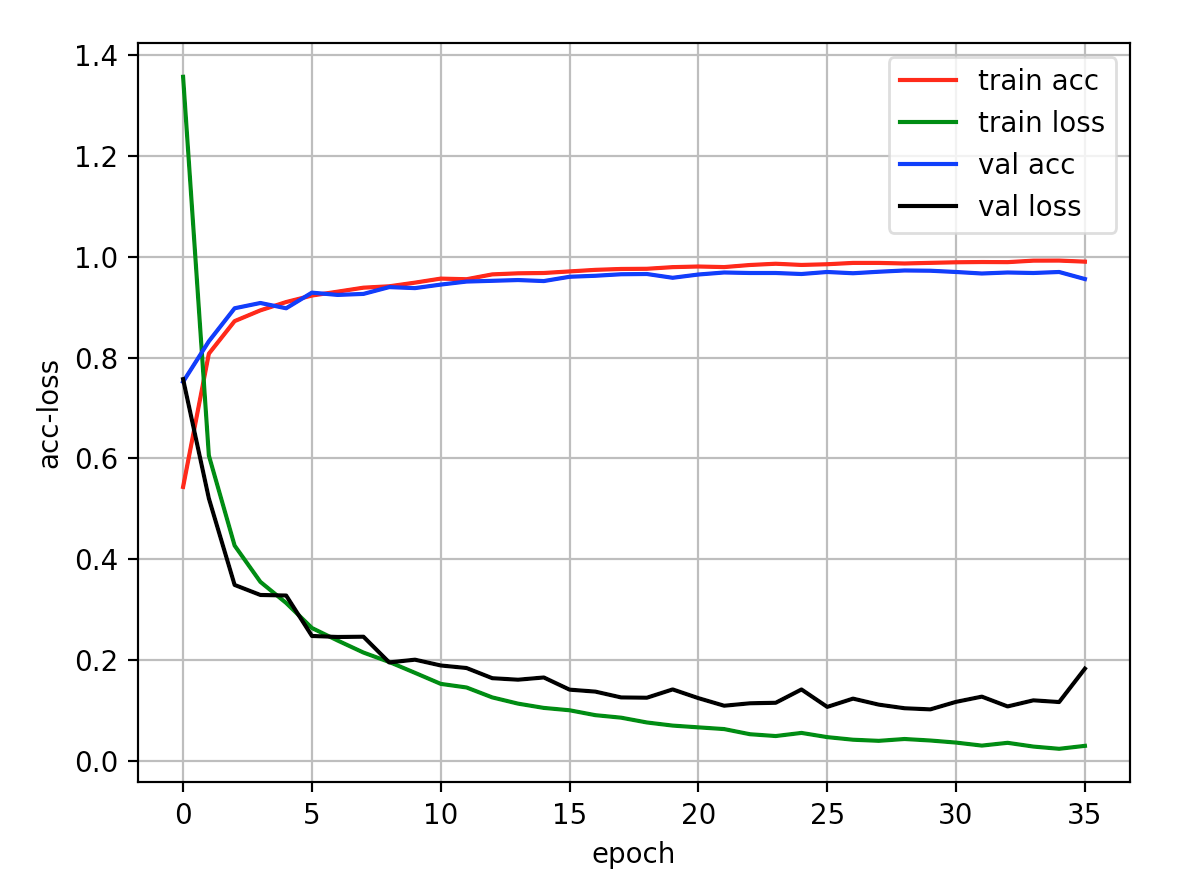
\includegraphics[scale = 0.3]{sgd_2.png}
\caption{Loss and Accuracy curve for SGD optimizer with Conv-dense model}
\end{minipage}
\begin{minipage}[t]{0.48\textwidth}
\centering
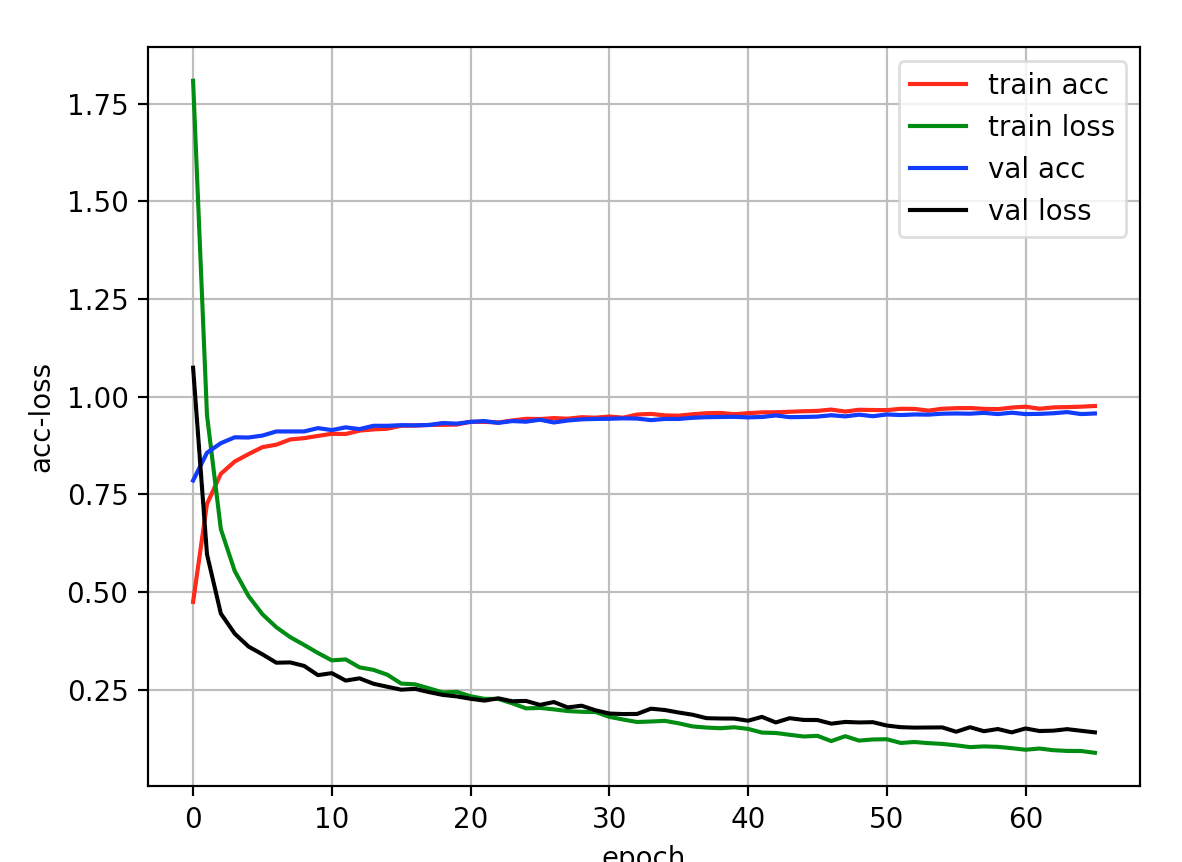
\includegraphics[scale = 0.3]{adadelta_2.png}
\caption{Loss and Accuracy curve for SGD optimizer with Conv-dense model}
\end{minipage}
\end{figure}

\begin{figure}[htbp]
\centering
\begin{minipage}[t]{0.48\textwidth}
\centering
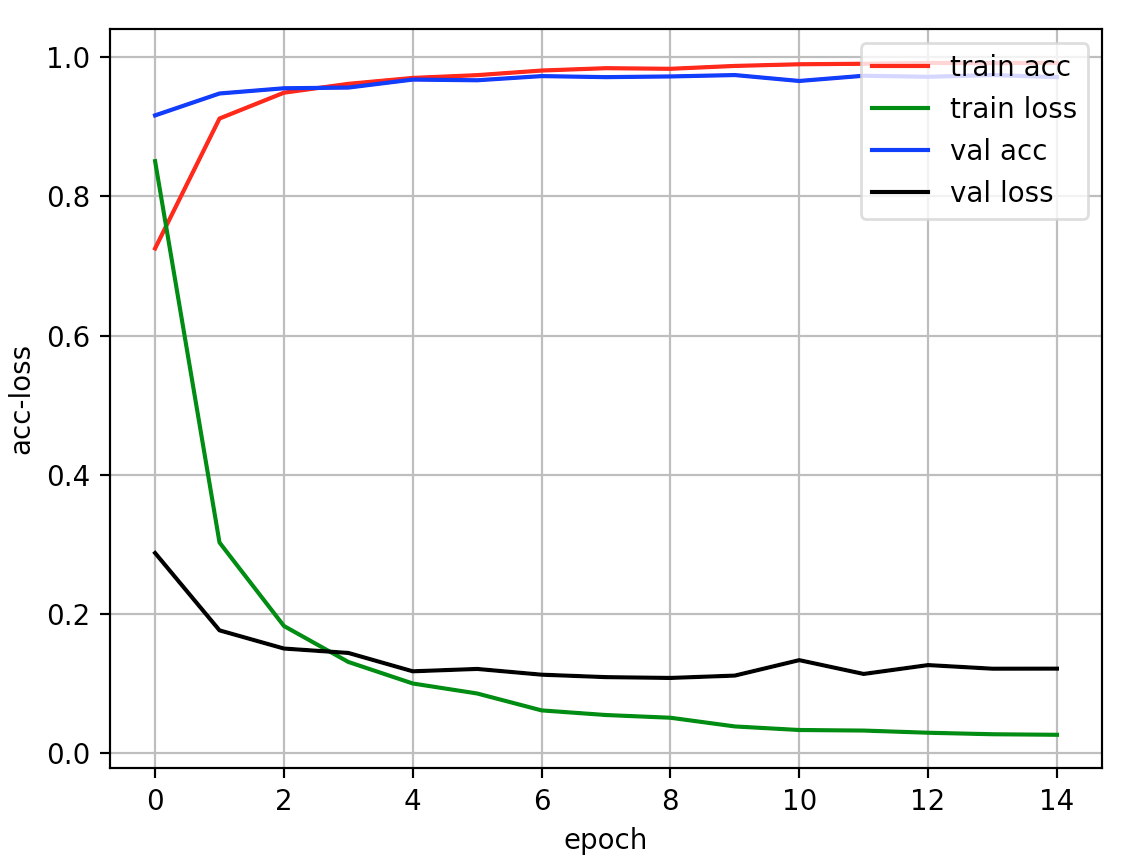
\includegraphics[scale = 0.3]{adam_2.png}
\caption{Loss and Accuracy curve for Adam optimizer with Conv-dense model}
\end{minipage}
\begin{minipage}[t]{0.48\textwidth}
\centering
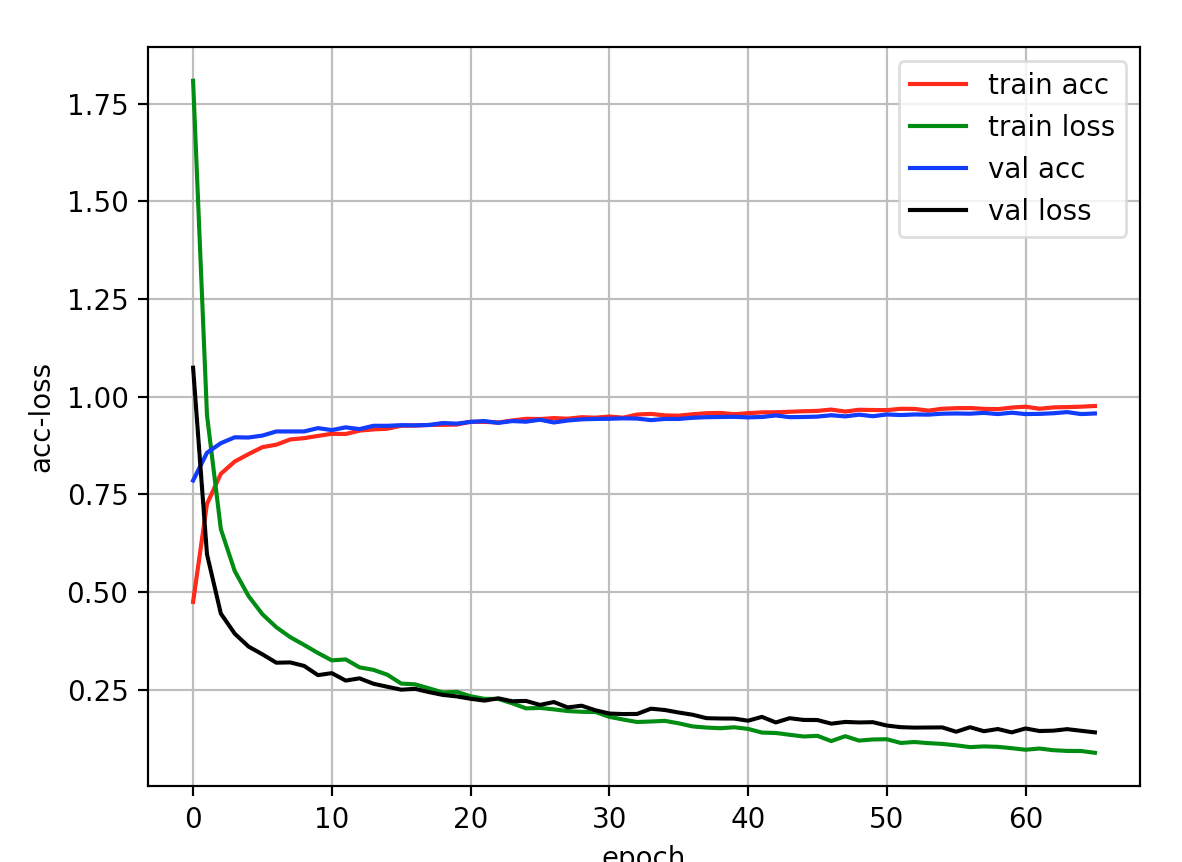
\includegraphics[scale = 0.3]{adadelta_2.png}
\caption{Loss and Accuracy curve for Adadelta optimizer with Conv-dense model}
\end{minipage}
\end{figure}

\subsubsection*{Conv-Conv-dense model}

This model contains two convlution layers with one max pooling layer. Then I use one fully connected layers to make the shape have the same form of the final output. Figure 12 shows the structure of this model.

\begin{figure}[htbp]
    \centering
    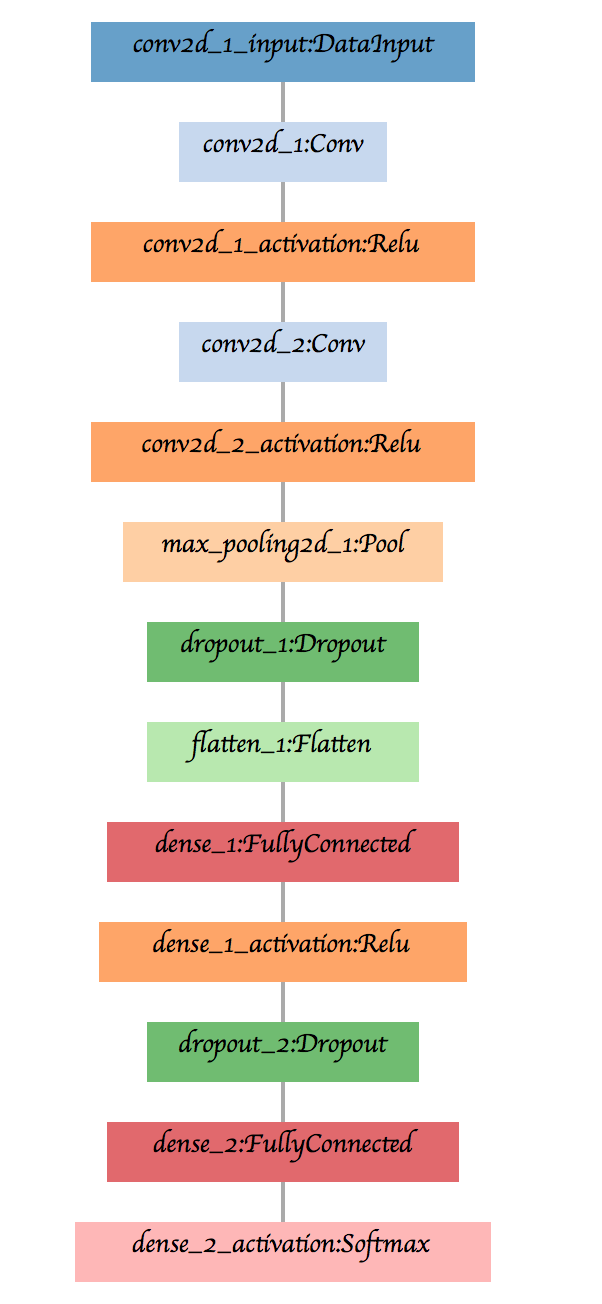
\includegraphics[scale = 0.5]{model_3.png}
    \caption{Model architecture for conv-conv-dense model}
    \label{fig12}
\end{figure}

The parameters like $kernel_size$, $pool_size$ keep the same as the two experiments. There are 5 hyper parameters: $lr$, $hidden_layers$, $Dropout_rate$, $filter1$ and $filter2$. I set the values by trying different values and find the best ones.

Table 5 shows the values of these parameters.

\begin{table}[htbp]
    \caption{Values of parameters for Conv-Dense model}
    \centering
    \begin{tabular}{|l|c|}
    \hline
         Parameters & values \\ \hline
         lr & 0.2 \\
         batch\_size & 150 \\
         hidden\_layer & 128  \\
         Dropout\_rate & 0.5 \\
         filter1 & 64 \\
         filter2 & 32\\
         \hline
    \end{tabular}
    \label{table5}
\end{table}

Table 6 shows the result of different optimizers with the same experimental condition. Also, the lr of adam and adagrad is 0.002 and 0.02.

\begin{table}[ht]
    \caption{Result on 3 optimizers}
    \centering
    \begin{tabular}{|l|c|c|c|c|}
    \hline
         Optimizer  & Adaelta & SGD & Adam & Adagrad\\ \hline
         Convergence Rate(epoches) &  104 & 36 & 17 &  26\\ \hline
         train acc & 97.85\% & 98.84\% & 98.43\% & 99.10\% \\
         train loss & 0.0702 & 0.0376 & 0.0475 & 0.0282\\ \hline
         val acc & 97.10\% & 97.70\% & 97.85\% & 97.80\% \\
         val loss & 0.0989 & 0.0859 & 0.0805 & 0.0830 \\ \hline
         test acc & 97.74\% & 98.09\% & 98.05\% & 98.24\%\\
         test loss & 0.0732 & 0.0672 & 0.0671 & 0.0612\\ \hline
    \end{tabular}
    \label{table6}
\end{table}

Figure 13 to Figure 16 show the curve of Loss and Accuracy as before.

\begin{figure}[htbp]
\centering
\begin{minipage}[t]{0.48\textwidth}
\centering
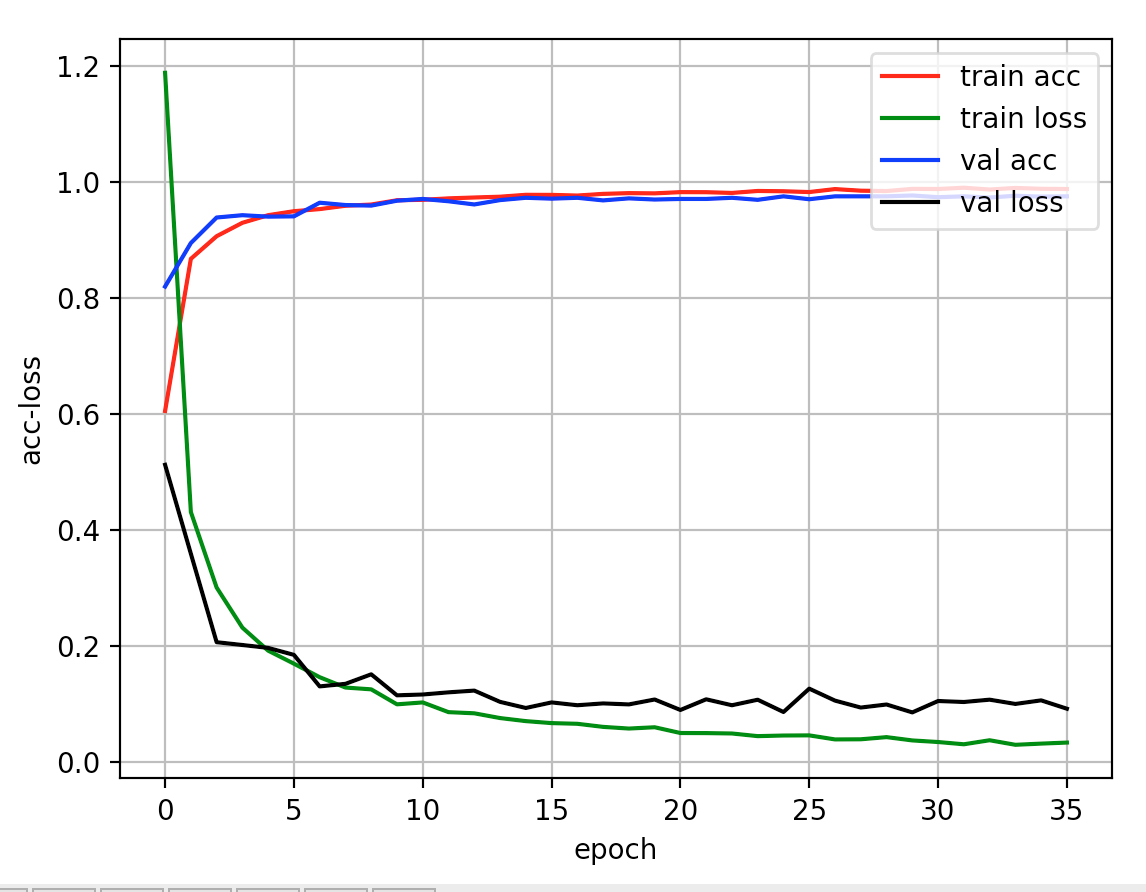
\includegraphics[scale = 0.3]{sgd_3.png}
\caption{Loss and Accuracy curve for SGD optimizer with Conv-conv-dense model}
\end{minipage}
\begin{minipage}[t]{0.48\textwidth}
\centering
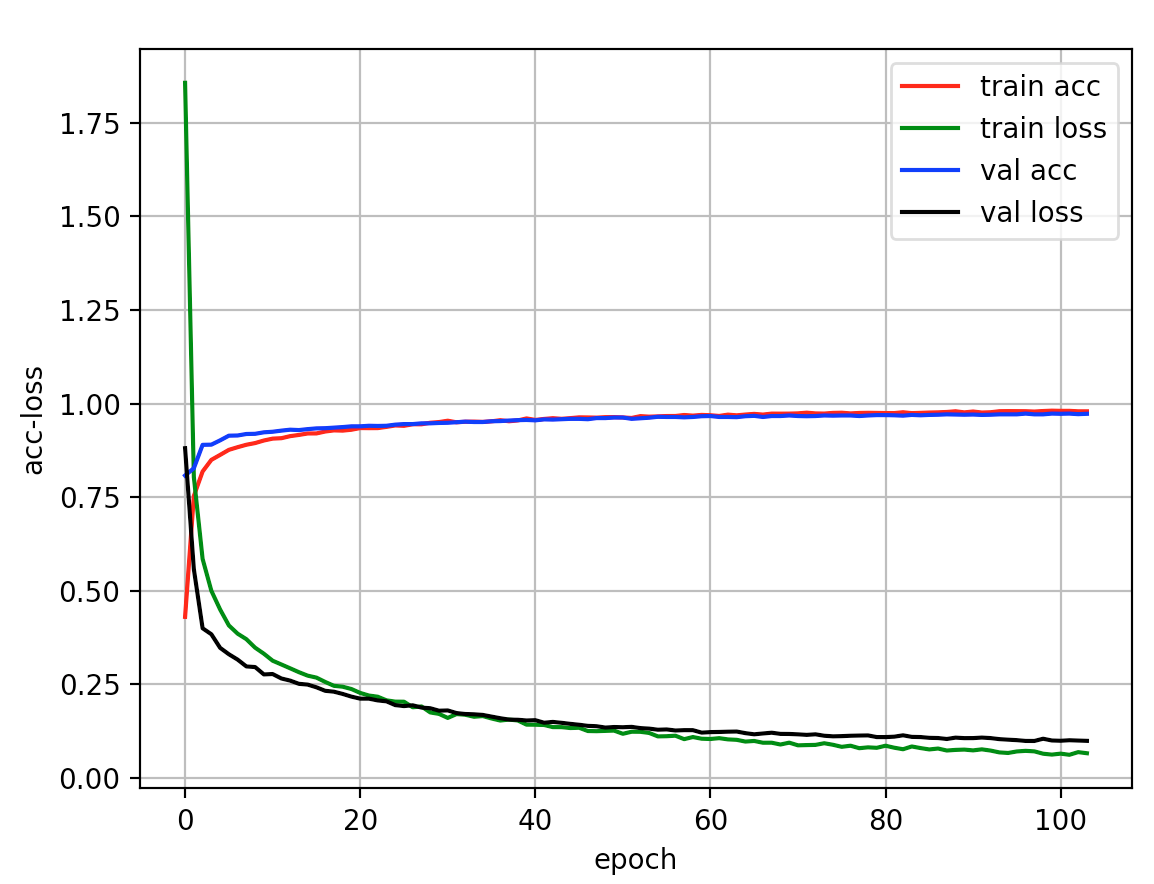
\includegraphics[scale = 0.3]{adadelta_3.png}
\caption{Loss and Accuracy curve for SGD optimizer with Conv-conv-dense model}
\end{minipage}
\end{figure}

\begin{figure}[htbp]
\centering
\begin{minipage}[t]{0.48\textwidth}
\centering
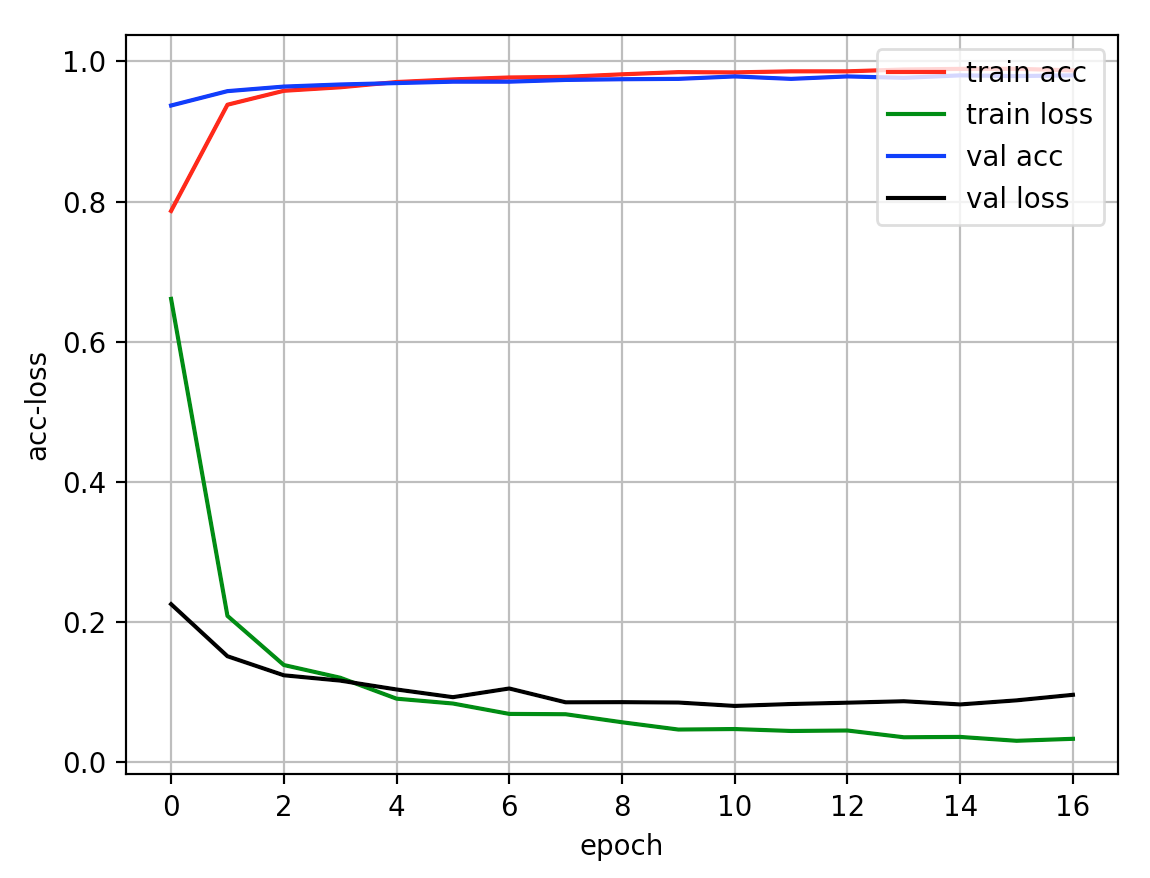
\includegraphics[scale = 0.3]{adam_3.png}
\caption{Loss and Accuracy curve for Adam optimizer with Conv-conv-dense model}
\end{minipage}
\begin{minipage}[t]{0.48\textwidth}
\centering
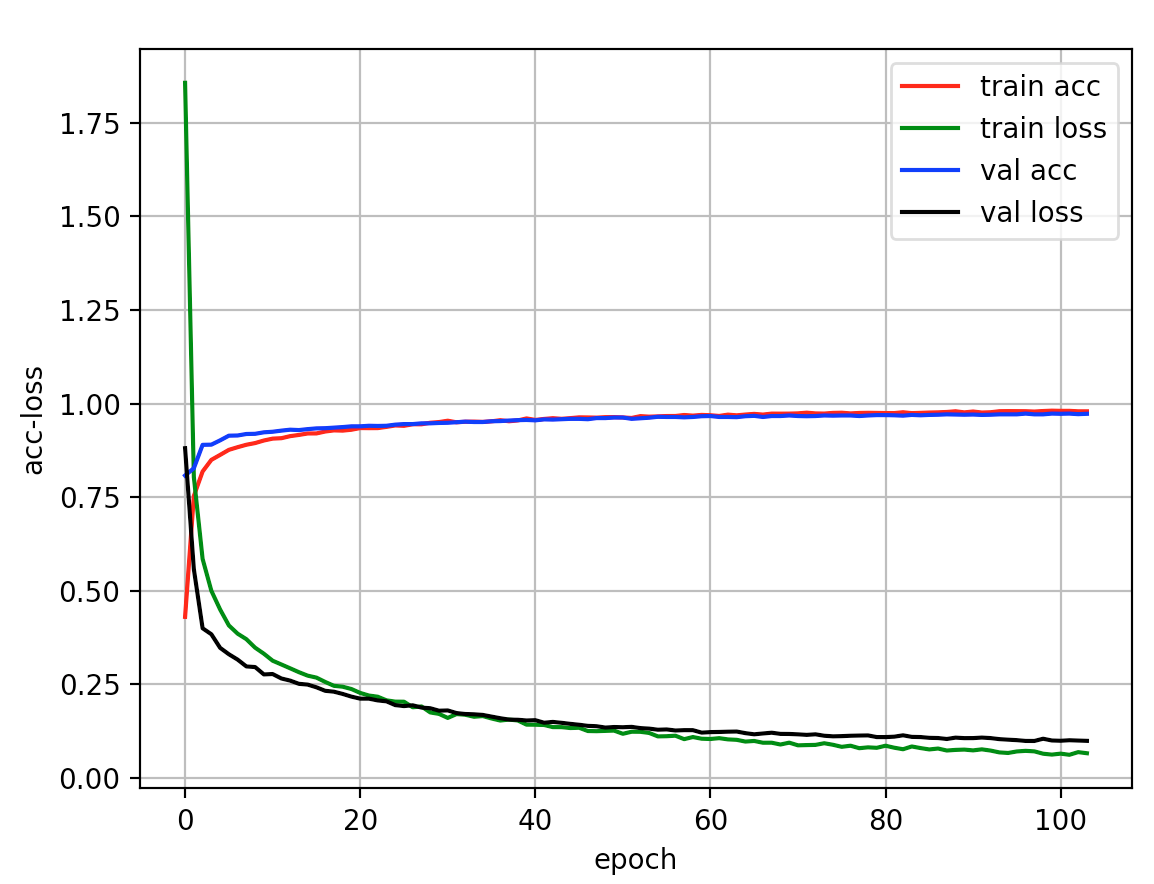
\includegraphics[scale = 0.3]{adadelta_3.png}
\caption{Loss and Accuracy curve for Adadelta optimizer with Conv-conv-dense model}
\end{minipage}
\end{figure}



\subsubsection*{Other experiments and some conclusions}

As mnist dataset is quite a small and easy dataset, two layers of CNN can work very well for it. If we build more complex models, the data is insufficient to train it and we may also face the problem of gradient disappearance. To verify this point, I also build a 5-layer CNN model with 2 fully-connected layers. I trained this model and the result went a little higher: about 98.50\% in test set. But the training time is about 4 times compared to the conv-conv-dense model. So I think it is worthless to train such a deep model as the 3rd model could represent the data well.

Besides, I also tried to include all the 60,000 samples as the training set, the accuracy in the test set can reach to 99.45\% for the 3rd model.


From these experiments, we cam get several conclusions:
\begin{enumerate}
    \item For all the 4 optimizers, they all work for this task, but the $Adam$ had a better performance with less training time and relatively higher accuracy.
    \item CNN network is sensitive to the amount of data. More data can lead to more effective model. The reason lies that the parameters need more samples to train.
    \item Compared with fully-connected model, CNN model can represent the data better. The reason is that CNN can extract and select local features which is the real feature we need for this task.
    \item Usually, complicated models can solve complicated problems. However, when building the model, we need to take the size of data set and the size of the problem into consideration. Then we can choose a suitable model that plays a good trade-off between training time and training result.
    \item The 2nd model and the 3rd model is more robust than the 1st one. We can see, when the accuracy for the training set goes up to 99\%, the accuracy of test set is only about 96\%. When using the Conv-conv-dense model, the difference between $train_acc$ and $test_acc$ reduced to less than 1\%, which says the model and the features are effective.
\end{enumerate}

\subsubsection*{Original Codes}
Codes for dense model:
\begin{lstlisting}
from __future__ import print_function
import keras
from keras.datasets import mnist
from keras.models import Sequential
from keras.layers import Dense, Dropout, Flatten
from keras.layers import Conv2D, MaxPooling2D
from keras import backend as K
from keras.callbacks import EarlyStopping, ModelCheckpoint
from keras.models import load_model
from keras.optimizers import Adadelta, SGD, Adagrad, Adam


import numpy as np
import matplotlib.pyplot as plt

#const
num_classes = 10
epochs = 200
train_patience = 6
model_name = 'dense.h5'


batch_size = 150
lr = 0.1
hidden_layer1 = 512
hidden_layer2 = 256
Dropout_rate = 0.3

class LossHistory(keras.callbacks.Callback):
    def on_train_begin(self, logs={}):
        self.losses = {'batch':[], 'epoch':[]}
        self.accuracy = {'batch':[], 'epoch':[]}
        self.val_loss = {'batch':[], 'epoch':[]}
        self.val_acc = {'batch':[], 'epoch':[]}

    def on_batch_end(self, batch, logs={}):
        self.losses['batch'].append(logs.get('loss'))
        self.accuracy['batch'].append(logs.get('acc'))
        self.val_loss['batch'].append(logs.get('val_loss'))
        self.val_acc['batch'].append(logs.get('val_acc'))

    def on_epoch_end(self, batch, logs={}):
        self.losses['epoch'].append(logs.get('loss'))
        self.accuracy['epoch'].append(logs.get('acc'))
        self.val_loss['epoch'].append(logs.get('val_loss'))
        self.val_acc['epoch'].append(logs.get('val_acc'))

    def loss_plot(self, loss_type):
        iters = range(len(self.losses[loss_type]))
        plt.figure()
        # acc
        plt.plot(iters, self.accuracy[loss_type], 'r', label='train acc')
        # loss
        plt.plot(iters, self.losses[loss_type], 'g', label='train loss')
        if loss_type == 'epoch':
            # val_acc
            plt.plot(iters, self.val_acc[loss_type], 'b', label='val acc')
            # val_loss
            plt.plot(iters, self.val_loss[loss_type], 'k', label='val loss')
        plt.grid(True)
        plt.xlabel(loss_type)
        plt.ylabel('acc-loss')
        plt.legend(loc="upper right")
        plt.show()



# input image dimensions
img_rows, img_cols = 28, 28

# the data, shuffled and split between train and test sets
data_file = np.load('mnist.npz')
x_train, y_train, x_test, y_test = data_file['x_train'],data_file['y_train'],data_file['x_test'],data_file['y_test']


if K.image_data_format() == 'channels_first':
    x_train = x_train.reshape(x_train.shape[0], 1, img_rows, img_cols)
    x_test = x_test.reshape(x_test.shape[0], 1, img_rows, img_cols)
    input_shape = (1, img_rows, img_cols)
else:
    x_train = x_train.reshape(x_train.shape[0], img_rows, img_cols, 1)
    x_test = x_test.reshape(x_test.shape[0], img_rows, img_cols, 1)
    input_shape = (img_rows, img_cols, 1)

x_train = x_train.astype('float32')
x_test = x_test.astype('float32')
x_train /= 255
x_test /= 255
print('x_train shape:', x_train.shape)
print(x_train.shape[0], 'train samples')
print(x_test.shape[0], 'test samples')

# convert class vectors to binary class matrices
y_train = keras.utils.to_categorical(y_train, num_classes)
y_test = keras.utils.to_categorical(y_test, num_classes)

###start codes
model = Sequential()
model.add(Flatten(input_shape=input_shape))
model.add(Dense(hidden_layer1,activation = 'relu'))
model.add(Dropout(Dropout_rate))
model.add(Dense(hidden_layer2, activation='relu'))
model.add(Dropout(Dropout_rate))
model.add(Dense(num_classes, activation='softmax'))

model.compile(loss=keras.losses.categorical_crossentropy,
              optimizer=Adagrad(lr = 0.001),
              metrics=['accuracy'])



history = LossHistory()
callbacks = [
  EarlyStopping(monitor='val_loss', patience=train_patience, verbose=0),
  ModelCheckpoint(model_name, monitor='val_loss', save_best_only=True, verbose=0),
  history,
]

model.fit(x_train, y_train,
          batch_size=batch_size,
          epochs=epochs,
          verbose=1,
          validation_split = 0.2,
          callbacks = callbacks)

model = load_model(model_name)

score = model.evaluate(x_test, y_test, verbose=0)
print('Test loss:', score[0])
print('Test accuracy:', score[1])

history.loss_plot('epoch')

\end{lstlisting}

Codes for Conv-dense model:
\begin{lstlisting}
###only show the different codes
model = Sequential()
model.add(Conv2D(filter_num, kernel_size=(kernel_size, kernel_size),
                 activation='relu',
                 input_shape=input_shape))
model.add(MaxPooling2D(pool_size=(pool_size, pool_size)))
model.add(Flatten())
model.add(Dense(hidden_layer1,activation = 'relu'))
model.add(Dropout(Dropout_rate))
model.add(Dense(hidden_layer2, activation='relu'))
model.add(Dropout(Dropout_rate))
model.add(Dense(num_classes, activation='softmax'))
\end{lstlisting}

Codes for Conv-conv-dense model:
\begin{lstlisting}
##only show the different codes
model = Sequential()
model.add(Conv2D(filter1, kernel_size=(kernel_size, kernel_size),
                 activation='relu',
                 input_shape=input_shape))
model.add(Conv2D(filter2, (kernel_size, kernel_size), activation='relu'))
model.add(MaxPooling2D(pool_size=(pool_size, pool_size)))
model.add(Dropout(Dropout_rate))
model.add(Flatten())
model.add(Dense(128, activation='relu'))
model.add(Dropout(Dropout_rate))
model.add(Dense(num_classes, activation='softmax'))

\end{lstlisting}

\section*{Secondary task: Camera resectioning}

\subsubsection*{Step 0: Get the corresponding points and their coordinates}

The most basic part of this task is to get the corresponding points. As described in the explanation, the distance between each two interfacing points is $7cm$. Take the corner as the polar point, then we can build a right-hand 3D coordinate system. Figure 17 shows the result of this 3D coordinate system. 

\begin{figure}[htbp]
    \centering
    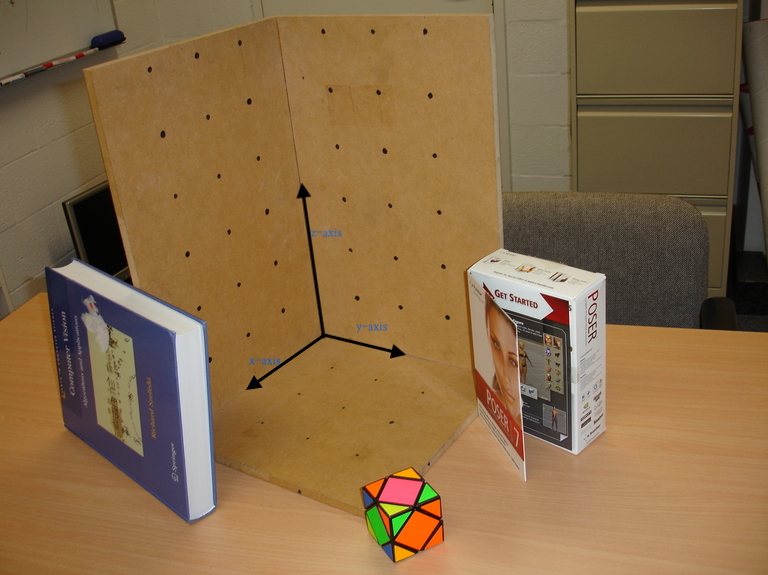
\includegraphics[scale = 0.35]{fig20.jpg}
    \caption{3D coordinate system for task 2}
    \label{fig17}
\end{figure}

Then I select 12 points symmetrically. Their locations are showed below.

\begin{figure}[htbp]
    \centering
    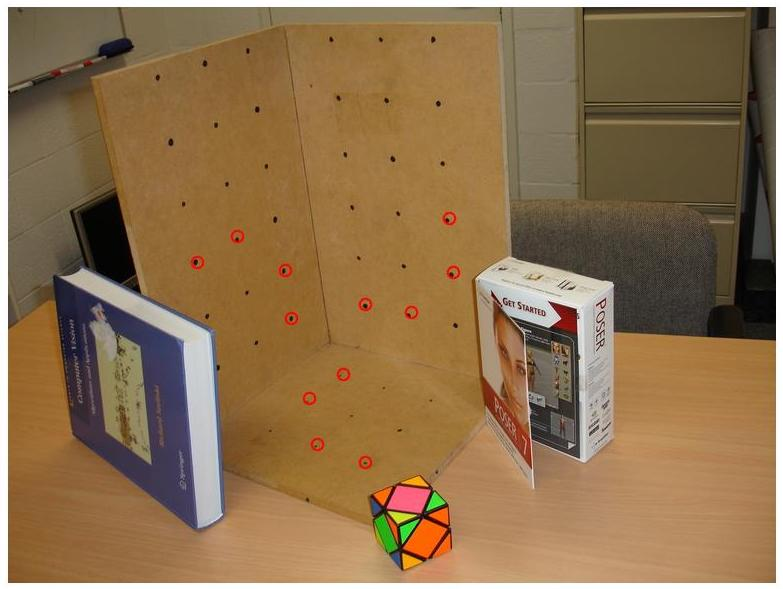
\includegraphics[scale = 0.35]{fig21.jpg}
    \caption{Selected points}
    \label{fig18}
\end{figure}

\subsubsection*{Step 1: Implement the calibration function}

From the slides of the lecture, we the key points in 3D DLT algorithm is to estimate P from matrix A, which is got from several pairs of corresponding points. Similar to Clab3, is given a pair of 3D-2D points, we can use a matrix P to describe their connections. $x = PX$ where $x$ is the 2D coordinates and $X$ is the 3D coordinates. That can also be expressed as: 

$$\begin{bmatrix}
u \\ v \\ 1 \end{bmatrix} = \left[ \begin{array}{ccc} p_{00} & p_{01} & p_{02} \\ p_{10} & p_{11} & p_{12} \\ p_{20} & p_{21} & p_{22} \\ p_{30} & p_{31} & p_{32} \end{array} \right] \times \left[ \begin{array}{c} X \\ Y \\ Z \\ 1 \end{array} \right]$$

After expose this equation, we can get following equations: 

$$\left [\begin{array}{ccc}
0^T & -X_i^T & v_iX_i^T \\ u_iX_i^T & 0^T & -u_iX_i^T
\end{array}\right] \left[ \begin{array}{c} p_1 \\ p_2 \\ p_3 \end{array} \right] = A_iP = 0 $$

From the lecture, we know that P is the smallest eigen vector of $V$ where $V$ is the SVD decomposition of A.

So, for this step, I first build A from the given points and then apply a SVD decomposition method to get C. The following shows the basic related codes:

\begin{lstlisting}
A = zeros(len*2,12);

for tmp = 1:len
   %get the 3D vertices and their 2D corresponding points
   X = XYZ(tmp,1);
   Y = XYZ(tmp,2);
   Z = XYZ(tmp,3);
   
   u = uv(tmp,1);
   v = uv(tmp,2);
   
   A(tmp*2-1,:) = [X,Y,Z,1,0,0,0,0,-u*X,-u*Y,-u*Z,-u];
   A(tmp*2,:) = [0,0,0,0,X,Y,Z,1,-v*X,-v*Y,-v*Z,-v];
end
[~,~,V] = svd(A);

C = V(:,end);
C = C/C(end);
C = reshape(C,[4 3]);
C = C';

\end{lstlisting}

Then we are required to show the distance between the projective points and the original points and the error of P. I take the mean-square error (MSE) of the points to represent the required error. Then I also plot the projective points of the 3D coordinates to have a visual detect.

The codes are listed below:

\begin{lstlisting}
imshow(im);
hold on;
plot(uv(:,1),uv(:,2),'ro');
hold on;
xyz1 = [XYZ,ones(tmp,1)]';
xy = C*xyz1;

xy(1,:) = xy(1,:)./xy(3,:);
xy(2,:) = xy(2,:)./xy(3,:);

distance = (xy(1:2,:) - uv').^2;
distance = mean(sum(distance));
disp(['Mean Square Error: ',num2str(distance)]);

plot(xy(1,:),xy(2,:),'g+');
\end{lstlisting}

\subsubsection*{Step 2: Test results on input images}

I choose the \emph{stereo2012a.jpg} as input image. The result of P and the visible result are shown below. 

$$P = \left[ \begin{array}{cccc} -6.0199 & 3.8788 & -2.1667 & 325.0822 \\ 1.3271 & -0.2787 & -7.3720 & 333.3063 \\ -0.0054 & -0.0050 & -0.0037 & 1.0000 \end{array} \right] $$

\begin{figure}[htbp]
    \centering
    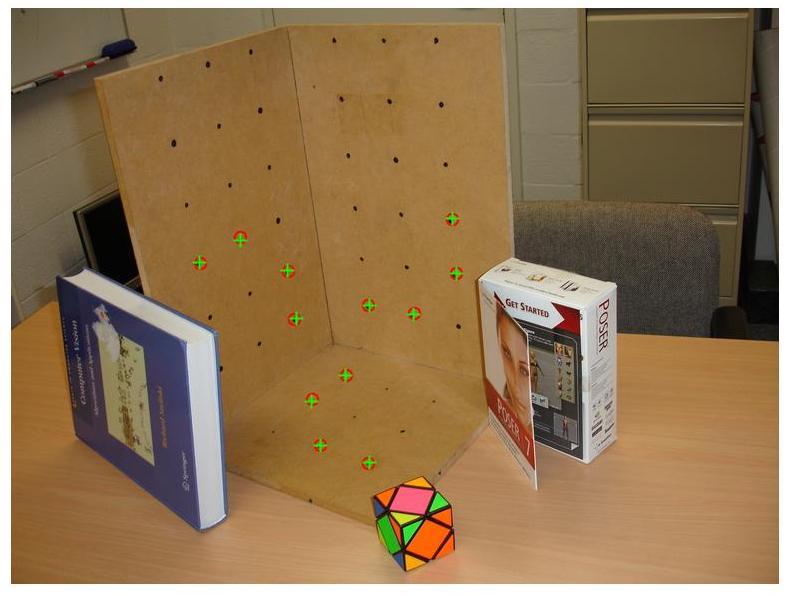
\includegraphics[scale = 0.35]{fig22.jpg}
    \caption{Visible result}
    \label{fig19}
\end{figure}

Here, the MSE is 2.2515. We can see directly that the result fits well for this image. The detailed result analysis will be released in the fourth part.

\subsubsection*{Rebuild K, R, t and focal based on P}
From the given codes, we can get the K, R, t from the given P matrix. I first have d look at the codes, it misses a function named $vgg\_rq()$. I think this function is used to get RQ decomposition of a matrix. So I wrote it on my own based the Matlab inbuilt $qr()$ function. The theory is easy to understand. If 
$$H = R\times Q$$
then $$inv(H) = inv(R\times Q) = Q'\times R^{-1}$$ 

Then I ran the codes with the P from the last part. However, I found an interesting thing, that is we know $P = K[R,t]$. But when I calculate P using the rebuilt K, R and t, they are not equal! I reanalyze the provided codes and found two confusing things.

\begin{lstlisting}
    if nargin < 2
      K = K / K(N,N);
      ...
\end{lstlisting}

Here, we noticed that if there is only one input element, K will be normalized. However, We did not normalize R in the same time. So at this situation, K*R is not equal to P[:3,:3].

Besides, the part of calculating t is not the same as what we learned in the lecture. 

From the lecture, we saw that 

$$P = K [R, t] = K[R, -RC] = [M, -MC]$$

In the provided codes, we get the 't' from

\begin{lstlisting}
  t = -P(:,1:N)\P(:,end);
\end{lstlisting}

Actually, here t is 'C' in the lecture. If we want to get t. we will left times -R. Thus, I changed the codes a little. The changed part are listed below.

\begin{lstlisting}
    %...
    if nargin < 2
      R = R * K(N,N);
      K = K / K(N,N);
    %...
    
    if nargout > 2
      t = -P(:,1:N)\P(:,end);
    end

    t = -R*t;
\end{lstlisting}

Then, running the codes, I can get the correct result. The results are as follows. Moreover, I found this code is widely used, maybe they have a different definition of 'K', 'R' and 't'. But here, I take what we learned as standard.

$$K = \left[ \begin{array}{ccc} 852.9772 & -6.6110 & 307.1738 \\ 0 & -853.1713 & 311.6108 \\ 0 & 0 & 1.0000 \end{array} \right] $$

$$R = \left[ \begin{array}{ccc} -0.0051 & 0.0064 & -0.0012 \\ -0.0035 & -0.0015 & 0.0073\\ -0.0054 & -0.0050 & -0.0037 \end{array} \right] $$

$$t = \left[ \begin{array}{c} 0.0208 \\ -0.0254 \\ 1.0000 \end{array} \right] $$

Now, $K\times [R, t]$ is equal to P.

Finally, we need to consider how to calculate the focal. I searched the slides, and found that the definition of K is:

$$K = \left[ \begin{array}{ccc} \alpha & \gamma & u_0 \\ 0 & \beta & v_0 \\ 0 & 0 & 1 \end{array} \right] $$

where 
$$\alpha = f_x; \beta = f_y/\sin{\theta}; \gamma = -f_x\cot{\theta}$$

So from K we can actually rebuild focal. I wrote the following codes to calculate the focal.

\begin{lstlisting}
    alpha = K(1,1);
    gama = K(1,2);
    thelta = acot(gama/-alpha);
    fx = abs(alpha);
    fy = abs(K(2,2)*sin(thelta));
    f = sqrt(fx^2+fy^2);
    disp(['fx: ',num2str(fx)]);
    disp(['fy: ',num2str(fy)]);
    disp(['focal: ',num2str(f)]);
\end{lstlisting}

The result is wield. It shows:
$$f_x = 852.9772$$
$$f_y = 853.1457$$
$$focal = 1206.4111$$

As the coordinates of the 3D points are based on $cm$ so the focal is about 12m! It must be wrong. But I do not have enough time to figure out the reason. I think the reason is probably the definition of 'K', 'R', 't' in the provided codes are different from what we learned.

Besides, the $\theta$ is equal to 89.5559 angle which is regular from the slides. The pitch angle is 90 angle.

\subsubsection*{Conclusion and result analysis}

From the visual analysis and MSE, I found the result of my codes is acceptable. However, there are still some errors. I think the reason may stands as follows:

\begin{enumerate}
    \item There are 12 pairs of points, when we calculating P, P cannot project every point in the correct location.
    \item When we select points using $ginput()$, the position of the 2D points are not that accurate.
    \item Matlab inbuilt function SVD uses a reiteration method to make the decomposition, it will also cause some error.
\end{enumerate}

The $Calibrate.m$ is listed in the next part. The other questions are answered / listed above.


\subsubsection*{Supportive codes}
\textbf{Main codes}
\begin{lstlisting}
close all;
clear all;
clc;

load data;

file_path = './CLAB5-Images/stereo2012a.jpg';
img = imread(file_path);

C = calibrate(img,XYZ,[u,v]);
[K, R, t] = vgg_KR_from_P(C);
disp('K = ');
disp(K);
disp('R = ');
disp(R);
disp('t = ');
disp(t);
%calculate focal
alpha = K(1,1);
gama = K(1,2);
thelta = acot(gama/-alpha);
fx = abs(alpha);
fy = abs(K(2,2)*sin(thelta));
f = sqrt(fx^2+fy^2);
disp(['fx: ',num2str(fx)]);
disp(['fy: ',num2str(fy)]);
disp(['focal: ',num2str(f)]);

\end{lstlisting}


\textbf{Calibrate.m}
\begin{lstlisting}
function C = calibrate(im, XYZ, uv)
%% TASK 1: CALIBRATE
%
% Function to perform camera calibration
%
% Usage:   K = calibrate(image, XYZ, uv)
%
%   Where:   image - is the image of the calibration target.
%            XYZ - is a N x 3 array of  XYZ coordinates
%                  of the calibration target points. 
%            uv  - is a N x 2 array of the image coordinates
%                  of the calibration target points.
%            C   - is the 3 x 4 camera calibration matrix.
%  The variable N should be an integer greater than or equal to 6.
%
%  This function plots the uv coordinates onto the image of the calibration
%  target. 
%
%  It also projects the XYZ coordinates back into image coordinates using
%  the calibration matrix and plots these points too as 
%  a visual check on the accuracy of the calibration process.
%
%  Lines from the origin to the vanishing points in the X, Y and Z
%  directions are overlaid on the image. 
%
%  The mean squared error between the positions of the uv coordinates 
%  and the projected XYZ coordinates is also reported.
%
%  The function should also report the error in satisfying the 
%  camera calibration matrix constraints.
[len,~] = size(uv);

A = zeros(len*2,12);

for tmp = 1:len
   %get the 3D vertices and their 2D corresponding points
   X = XYZ(tmp,1);
   Y = XYZ(tmp,2);
   Z = XYZ(tmp,3);
   
   u = uv(tmp,1);
   v = uv(tmp,2);
   
   A(tmp*2-1,:) = [X,Y,Z,1,0,0,0,0,-u*X,-u*Y,-u*Z,-u];
   A(tmp*2,:) = [0,0,0,0,X,Y,Z,1,-v*X,-v*Y,-v*Z,-v];
end
[~,~,V] = svd(A);

C = V(:,end);
C = C/C(end);
C = reshape(C,[4 3]);
C = C';

imshow(im);
hold on;
plot(uv(:,1),uv(:,2),'ro');
hold on;
xyz1 = [XYZ,ones(tmp,1)]';
xy = C*xyz1;

xy(1,:) = xy(1,:)./xy(3,:);
xy(2,:) = xy(2,:)./xy(3,:);

distance = (xy(1:2,:) - uv').^2;
distance = mean(sum(distance));
disp(['Mean Square Error: ',num2str(distance)]);

plot(xy(1,:),xy(2,:),'g+');

end
\end{lstlisting}


\textbf{$vgg\_rq.m$}
\begin{lstlisting}
function [ R, Q ] = vgg_rq( H )
[q,r] = qr(inv(H));
Q = q';
R = r^-1;
end
\end{lstlisting}






\begin{thebibliography}{9}
\bibitem{early_stopping} Prechelt and Lutz. \textit{Early Stopping - But When?}. Neural Networks: Tricks of the Trade (1998), 55--69. Springer Berlin Heidelberg, Berlin, Heidelberg.

\bibitem{dropout} Geoffrey E. Hinton and Nitish Srivastava and Alex Krizhevsky and Ilya Sutskever and Ruslan Salakhutdinov. \textit{Improving Neural Networks by Preventing Co-adaptation of Feature Detectors}. Computer Science (2012), 3(4): 212-223. 



\end{thebibliography}


\end{document}
